\subsection{Search}
This subsection will allow users to search for playlists on their music accounts through Synthify.

\begin{figure}[h!]
	\centering
 	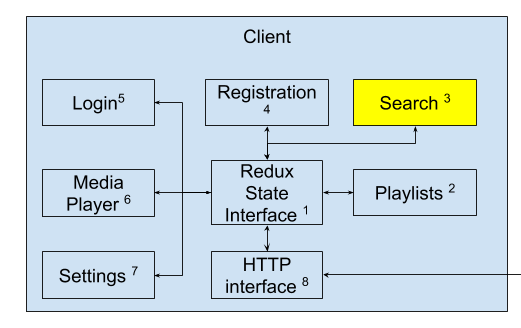
\includegraphics[width=0.60\textwidth]{images/client/client_search.png}
 	\caption{Search subsystem}
\end{figure}

\subsubsection{Subsystem Hardware}
No specific hardware will be used for searching.

\subsubsection{Subsystem Operating System}
No OS required. This will run through supported browsers such as Chrome 42 and Firefox 39.

\subsubsection{Subsystem Software Dependencies}
We will be using React.js 16.8.0-alpha, React-Router 4.3, Material-UI v3.9.0

\subsubsection{Subsystem Programming Languages}
JavaScript ES6 will be used.

\subsubsection{Subsystem Data Structures}
A fetch request will be made to the server. It will return an array of hashmaps that contains information such as artist name, song title, cover art and more.

\newpage
